\section{Design}
\label{sec:design}

\system infers efficient layouts for dense representations of recursive
datatypes. \system's key idea is that the best data layout should match the way
a program accesses these data.
%
\secref{sec:overview} shows how this idea reduces to finding an
ordering of fields in data constructors. The ordering must align with the
order a function accesses those fields, in which case the optimization improves
performance of the function.

To find a better layout for a datatype in the single-function case, \system first analyzes possible executions of the function and their potential for field accesses. In particular, \system takes into account (a) the various paths through a function, each of which may access fields in a different order, and (b) dependencies between operations in the function, as in the absence of dependencies, the function can be rewritten to access fields in the original order, and that order will work best. \system thus constructs a control-flow graph (\secref{design:cfg}) and collects data-flow information (\secref{design:dfa}) to build a {\em field access graph}, a representation of the various possible orders in which a function might access fields (\secref{subsec:attributes} and \secref{design:fieldgraph}).

Once data accesses in a function are summarized in the field access graph, \system proceeds with synthesizing a data layout. \system incorporates knowledge about the benefits of sequential, strided access and the drawbacks of pointer chasing and backtracking to define an abstract cost model. The cost model allows to formulate an integer linear program whose optimal solution corresponds to a layout that minimizes the cost according to that model (\secref{design:genconstraints}).

The remainder of this section walks through this design in detail, and discusses how to extend the system to handle multiple functions that use a datatype (\secref{design:global}).

\subsection{\system's Language}
\system{} operates on the language \systemlang{} given in \figref{fig:grammar}.


\systemlang{} is a first-order, monomorphic, call-by-value functional language
with algebraic datatypes and pattern matching.
%
Programs consist of a series of datatype definitions, function definitions, and a main expression.
%
\systemlang{}'s expressions use A-normal form~\cite{ANF}.
%
The notation $\vectorize{x}$ denotes a vector $ [x_1, \ldots, x_n] $ and $\vectorize{x_{\ind}}$
the item at position $\ind$.
%
\systemlang{} is an intermediate representation (IR) used towards the front end in the Gibbon compiler.
The monomorphizer and specializer lower a program written in a polymorphic, higher-order subset of Haskell\footnote{With strict evaluation semantics using \il{-XStrict}.} to \systemlang{},
and then location inference is used to convert it to the {\em location calculus} (LoCal) code next~\cite{Local}.
%
It is easier to update the layout of types in \systemlang{} compared to LoCal,
as in \systemlang{} the layout is implicitly determined by the ordering of fields,
whereas the later LoCal IR makes the layout explicit using locations and regions (essentially, buffers and pointer arithmetic).

\begin{figure}[t]
	\small
	

\begin{displaymath}
  \begin{aligned}
  &\DC \in \; \textup{Data Constructors},\:\: \TYP \in \; \textup{Type Constructors},
  \:\: \var, \yvar,\fvar \in \; \textup{Variables}%% ,\:\:
%%   \loc, \locreg{l}{r} \in \; \textup{Symbolic Locations},\\
%%   &\reg \in \; \textup{Regions},\:\: \ind, \indj \in \; \textup{Region Indices},\\
%%   &\concreteloc{r}{i}{l} \in \; \textup{Concrete Locations}
  \end{aligned}
\end{displaymath}
\begin{displaymath}
  \begin{aligned}
    \textup{Top-Level Programs} && \PROG && \gramdef & \vectorize{\DD} \;; \vectorize{\FD} \;; \EXPR \\
    \textup{Field of a Data Constructor} && \fields && \gramdef & \sTYP  \\
    \textup{Datatype Declarations} && \DD && \gramdef & \DATA\;\TYP = \vectorize{\DC \; \vectorize{\fields}\;} \\
    \textup{Function Declarations} && \FD && \gramdef & \fvar : \vectorize{\TYP} \ARROW \TYP ; \fappnoloc{\vectorize{\var}} = \EXPR \\
    %% \textup{Located Types} && \hTYP && \gramdef & \tyatlocreg{\TYP}{\loc}{\reg} \\
%%     \textup{Type Scheme} && \TS && \gramdef &
%%       \forall _{\vectorize{\locreg{l}{r}}}.
%%       \vectorize{\hTYP} \ARROW \hTYP \\
    \textup{Values} && \VAL && \gramdef & \var \\ %% \gramor \concreteloc{\reg}{\ind}{\locreg{\loc}{\reg}}
    \textup{Expressions} && \EXPR && \gramdef & \VAL\\[-5pt]
%%     && && \gramor & \fappnoloc{\vectorize{\VAL}} \\
%%     && && \gramor & \dataconnoloc{\DC}{\vectorize{\VAL}}\\
%%     && && \gramor & \copynoloc{\vectorize{\VAL}}\\
    && && \gramor & \letpack{\var:\TYP}{\fappnoloc{\vectorize{\VAL}}}{\EXPR} \\
    && && \gramor & \letpack{\var:\TYP}{\dataconnoloc{\DC}{\vectorize{\VAL}}}{\EXPR} \\
%%     && && \gramor & \letloc{\locreg{\loc}{\reg}}{\LE}{\EXPR} \\
%%     && && \gramor & \letreg{\reg}{\EXPR} \\
    && && \gramor & \case{\VAL}{\vectorize{\pat}} \\
    \textup{Pattern} && \pat && \gramdef &
    \caseclause{\datacon{\DC}{}{(\vectorize{\var : \TYP})}}{\EXPR} \\
%%     \textup{Location Expressions} && \LE && \gramdef
%%     & \startr{\reg} \\
%%     && && \gramor & (\locreg{\loc}{r} + 1) \\
%%     && && \gramor & \afterl{\hTYP}   \\        
%%     \textup{Copying Calls} && \cpy && \gramdef & \copyPacked{\var:\hTYP}
  \end{aligned}
\end{displaymath}

	\normalsize
        \caption{\new{Simplified grammar for a first-order, monomorphic functional language
            that \system operates on. \auditme{The full implementation includes more primitive datatypes, and built in primitives (such as a copy primitive).}}}
	%% \caption{Grammar definition of \system. This represents a
%%           point in compilation (1) with explicit locations, (2) after
%%           monomorphization. Functions are first order and the only
%%           remaining polymorphism is {\em location polymorphism}.}
	\label{fig:grammar}  
\end{figure}

%
% \csk{not sure if this phase ordering blurb is necessary...}
%
%In the remainder of this section, we describe the components of \system{}'s design in turn.

%
%% The remainder of this section is organized as follows, section~\ref{design:cfg} describes how we generate the control flow graph, section~\ref{design:fieldgraph} discusses how we generate the field access graph from the control flow graph,
%% {section~\ref{design:genconstraints} describes our cost model and how we obatain a minimum-cost ordering using
%% constraint solving.}
%% %% Section~\ref{design:genconstraints}, ~\ref{design:ilp} describe the constraint generation process and how we solve it using the ILP solver.
%% %% Finally, section~\ref{design:shufflefields} talks about the compiler pass that reorders the fields based on the locally optimal field ordering.

%% \note{RN: There's a lot of repetetion here. It might help to spell out the goal of each section in a small note at the top, and think through redundancy at that level.}

%% \subsection{Preliminaries}
%% \vs{Goal: Define all what a packed type is, what Algebraic data types are, fields, data constructors and grammar notation to make the user familiar with all the components of the analysis we are about to do. }
%% \begin{figure}[]
%% 	\begin{lstlisting}[ ]
	
%% 	data Tree a = Leaf a 
%% 	            | Node a (Tree a) (Tree a)
	
	

%% 	\end{lstlisting}
%% 	\caption{A packed data type in \system}
%% 	\label{lstlisting:packedtype}
%% \end{figure}

%% A \textit{packed type} (for example \textit{BlogList} in figure~\ref{fig:blog-traversal} and \textit{Tree} in figure~\ref{lstlisting:packedtype}) in \system is a data type whose values are serialized at contiguous addresses in memory.  As mentioned in the \secref{sec:overview}, the main motivation for such an in-memory serialization is to get the benefits of compactness, spatial locality and a predictable prefetch.
%% %
%% Still, where a traversal function doesn't touch all data, the compiler inserts necessary shortcut pointers (random access pointers) to different fields as required. This avoids generating dummy traversals.
%% \rn{Already covered...}

%% In the absence of such shortcut pointers, the traversal walks over unnecessary data by generating dummy traversals to reach the beginning of the desired location in the memory buffer. This doesn't preserve the asymptotic complexity of the program. Short cut pointers allow constant time access to data demanded by the function potentially ``out of the order'' it is serialized in memory. 

%% By matching the layout of the fields of a data type in memory to the traversal order of the function consuming it, 
%% we are optimizing the placement \textit{and} quantity of such shortcut pointers. At a high level, the layout of the data type should be such that it minimizes unnecessary {cursor} movement in the serialized buffer. This results in better locality and prefetching which enhances performance. Section~\ref{design:genconstraints} concretely defines such \textit{unnecessary movement} by encoding it in a cost model which is used to drive the layout optimization of the data type in memory. 

%% Defining a \textit{packed type} in \system can be done by using the keyword \textit{data} which allows the user to introduce data constructors to define the existence of different values that the packed type can take.
%% \rn{Definitely already covered!}
%% %
%% A packed type can have multiple such data constructors and each data constructor introduces different fields within itself which may be scalars or recursive fields.

%% Data constructors behave like function calls that take \textit{fields} of
%% some data {type variant as inputs and construct a value of that type}.
%% (Of course, any decent compiler open-codes the constructor primitives, not performing an actual runtime function call.)
%% %
%% We refer to scalar fields as primitive
%% types such as integers, floats and bools and non-scalar types are
%% \textit{packed} and potentially recursive fields.

%% \note{csk: specify that \system has 1-byte boolean values, but grammar doesn't include them for simplicity. can replicate booleans with case expressions of course.}
%% \note{csk: I've preserved the copy primitive in the grammar but it doesn't seem super relevant to marmoset.}

%% In our grammar, \figref{fig:grammar}, a data type of type $\tau$ is represented as $\DD$.  A data type can either be packed, unpacked, boxed or unboxed. However for our discussion, we assume its always \textit{packed and unboxed}. There can be multiple data constructors $\vectorize{\sDC}$ for a packed type $\DD$. Each data constructor $\sDC$ has some fields $\vectorize{\fields}$ of type $\vectorize{\sTYP}$ as shown in the grammar.

%% Given a program $\PROG$, it is constructed out of multiple data type declarations($\vectorize{\DD}$), functions($\vectorize{\FD}$) and expressions($\EXPR$). For a given program and function tuple $(\PROG, \FD)$ where the function $\FD$ consumes some data type $\DD$. We want to locally optimize the fields of the data constructors of $\DD$ for the function $\FD$. Hence for each data constructor $\sDC$ of the packed data type with fields $\vectorize{\fields}$ we want to find a total ordering on the fields of each data constructor such that it minimizes some costs and maximizes the performance of function $\FD$ that consumes the data type $\DD$.

%% \note{Need a discussion somewhere of how an entire program, with a control-flow graph of multiple functions, is handled.}

%% A programmer can write a program in \system using a subset of Haskell including polymorphic types. While compiling this language down to C, \system converts the higher-order, polymorphic language to a monomorphized intermediate representation with concrete types. There are a series of optimization passes including \lstinline{flatten} which flattens the intermediate representation and generated code in static single assignment, three address form. In order to find such an ordering, we analyze the function body of $\FD$ at the flattened level of the IR and gather the access patterns of the fields $\vectorize{\fields}$ for a data constructor $\sDC$ whose performance we are optimizing.

%% To orchestrate such an analysis, we construct a control flow graph for function $\FD$ after flattening the code in Gibbon's monomorphic IR\csk{edit due to grammar change.}\footnote{Called L1 in the implementation.}. We then use the control flow graph to construct a field access graph that captures the access patterns of the fields for a particular data constructor. Hence in our design, for a particular function, each data constructor $\sDC$ has an associated field access graph. This field access graph has the fields for that particular data constructor as vertices and directed edges between the vertices represent a temporal access between the two fields: {that is, both fields are accessed, and one is before the other.}

%% We use the field access graph to generate some constraints that we solve using an integer linear programming solver. The output of the solver is a mapping from the field to its locally optimal index in the data constructor that minimizes the costs when traversal $\FD$ traverses the data type.
  



% \begin{figure}[H]
% 		\begin{subfigure}[a]{\linewidth}
% 		\fontsize{10pt}{10pt}\selectfont
% 		\begin{flalign*}
% 	    	&\text{scalar types }  \ \  \epsilon  \ \  \text{\textbf{int} | \textbf{float} | \textbf{bool} | \textbf{char} }&\\
% 	    	&\text{non-scalar types } \ \  \epsilon  \ \  \text{\textbf{Vector (scalar types)} } &\\
% 	    	&\text{packed types} \ \  \epsilon \ \  
% 		\end{flalign*}
% 		\caption{Types in \system}
% 		\end{subfigure}
% \caption{Language definition of \system}
% \end{figure}

\subsection{Control-Flow Analysis}
\label{design:cfg}

%% \vs{Goal: Define how the control flow graph is build and its components / assumptions etc. }

\begin{algorithm}
    \caption{Control-Flow Graph Psuedocode}\label{alg:cfg}
    \begin{algorithmic}[1]
		\small
		\Input 
			\State exp: An expression in subset of \systemlang
			\State weight: The likelyhood of exp executing (\ie{} exp's inbound edge)
%			\State nodeId: A variable to track the id of cfg nodes
		\EndInput
		\Output
			\State A tuple of list of cfg nodes and the node id.
		\EndOutput
        \Function{ControlFlowGraph}{exp, weight}
            \algorithmiclet{nodeId = genFreshId()}
            \Switch{$exp$}
                \Case{LetE (v, ty, rhs) bod} \label{alg:cfg-let} 
					\algorithmiclet{(nodes, succId) = \Call{ControlFlowGraph}{bod, weight}}
					\algorithmiclet{newNode = (nodeId, (LetRHS (v, ty, rhs), weight), [succId])} \label{alg:cfg-likelihood}
					\State \Return (nodes ++ newNode, nodeId)
                \EndCase
%%                 \Case{IfE a b c} \label{alg:cfg-if}
%% 					\algorithmiclet{(n1, succB) = \Call{ControlFlowGraph}{b, weight/2}}
%% 					\algorithmiclet{(n2, succC) = \Call{ControlFlowGraph}{c, weight/2}}
%% 					\algorithmiclet{newNode = (nodeId, (a, weight), [succB, succC])}
%% 					\State \Return (n1 ++ n2 ++ [newNode], nodeId)
%%                \EndCase
				\Case{CaseE scrt cases} \label{alg:cfg-case}
					\algorithmiclet{(nodes, successors) = \Call{CfgCase}{weight/length(cases), cases}}
					\algorithmiclet{newNode = (nodeId, (scrt, weight), successors)}
					\State \Return (nodes ++ [newNode], nodeId)
				\EndCase
                \Case{VarE v}
                                        \algorithmiclet{newNode = (nodeId, (v, weight), [])}
					\State \Return ([newNode], nodeId)
                \EndCase
            \EndSwitch
        \EndFunction
    \end{algorithmic}
\end{algorithm}

%
We construct a control-flow graph with sub-expressions, and let-bound RHS's (right hand sides) of \systemlang{} as the nodes.
Algorithm~\ref{alg:cfg} shows the psuedocode for generating the control-flow graph.
%
\new{Because the syntax is flattened into A-normal form, there is no need to traverse within the RHS of a let expression.}
%
Edges between the nodes represent paths between expressions. The edges consist of {\em weights} (Line~\ref{alg:cfg-likelihood})
that represent the likelihood of a particular path being taken.
%%
%% csk: addressed
%% \rn{Not totally comfortable with calling this instruction
%%   level... since the ``instructions'' are arbitrary
%%   primitive-applications in the AST. It's not close to *machine*
%%   instruction level.}
%%   In this instruction-level control flow graph, each node is an instruction in three address form and edges exists between two nodes in the order of the execution of the program. The order of execution branches at \textit{if then else} instructions and \textit{case} instructions. For an \textit{if then else} condition, the order of execution branches in two different directions. For a case expression it branches $n$-ways, where $n$ is the number of different patterns that need to be matched for that particular case expression.
%
%% For this reason, we do not construct a traditional control-flow graph from the intermediate language but rather generate an instruction level control flow graph using the \textit{Data.Graph} library available with the \textit{containers} package in Haskell.
%Given a function definition, each sub-expression of the function body becomes a separate node in the \CFG.
An edge between two nodes indicates the order of the evaluation of the program.
%
% \footnote{The order of evaluation is straightforward to determine since \systemlang{} uses call-by-value semantics.}.
A node corresponding to a \il{let}-binding (Line~\ref{alg:cfg-let}) contains the bound expression
and has one outgoing edge to a node corresponding to the body expression.
%
A \il{case} expression (Line~\ref{alg:cfg-case}) splits the control flow $n$-ways,
where $n$ is the number of pattern matches.
{Outgoing edges of a node for a \il{case} expression have weights
  associated with them that correspond to the likelihood of taking a
  particular branch in the program.}
%% The likelihood parameter is threaded while generating the control flow graph, for the \textit{if then else} instruction since the control flow forks, the likelihood of each child edge becomes half, (\textit{likelihood of parent `div` 2} ). Similarly for a case instruction, each child's likelihood is assumed to be uniformly distributed for each of the possible match clauses.
%
%\mv{huh? why bring this up if we don't use the weights?}
%\ap{we now talk about it in the discussion, so let's skip it here}
% If available, dynamic profiling information can provide these weights.
% For the purposes of this paper, however, we find it is sufficient to use trivial placeholder weights: i.e. uniform weight over all branches.
% A node for a pattern match clause merely has an outgoing edge to its body expression.
%
Control flow terminates on a leaf \systemlang{} expression: a variable reference,
a data constructor or a function application.
% , for instance, either a data constructor, a function application, or a variable reference.

%% We plan to use dynamic techniques like profiling to calculate the actual frequency a particular path will be taken by the program at runtime. This depends on the input to the program.
%In the current implementation, a function call {\em does not} correspond to an edge to the callee's
%body in the \CFG, since \system{} only analyses one function at a time.
%
%In the future, we plan to extend our work to perform interprocedural analysis.
%
%\auditme{However, in the whole-program compilation setting (where types are already specialized and monomorphic), non-recursive functions can very often be inlined yielding a data traversal as a single recursive function.}

%
%\rn{This seems like a painful restriction to not extend the analysis across functions....}

\Figref{graph:running-cfg} shows the control-flow graph for the running example (\figref{fig:blog-traversal}).
%\new{(This example uses an \lstinline|if| expression, which is trivially desugared to \lstinline|case|.)}
%
{Each node corresponds to a sub-expression of the function \il{emphKeyword}.
%
The first \il{case} expression splits the control flow into two branches,
corresponding to whether the input list of blogs is empty or not.
%
The branch corresponding to the empty input list is assigned a probability $\alpha$, and
the other branch is assigned a probability $1 - \alpha$.
%
The next node corresponds to the pattern match \il{Blog content hashTags blogs'}.
%
Another two-way branch follows, corresponding to whether \il{keyword} occurs in
the \il{content} of this blog or not.
%
We assign the probabilities $\sigma$ and $1-\sigma$ to these branches respectively.
%
Note that as a result, the corresponding edges in the CFG have weights $(1 - \alpha)*\sigma$ and $(1 - \alpha)*(1 - \sigma)$, as the likelihood of {\em reaching} that condition is $(1 - \alpha)$.
%
Each of these branches terminate by creating a new blog entry with its content potentially updated.
%
In the current model, $\alpha$ and $\sigma$ are 0.5: they are uniformly distributed.
}
%

\auditme{One intuition for why realistic branch weights are not essential to \system's optimization is that accurate weights only matter if there is a trade off between control-flow paths that are best served by different layouts. The base cases (e.g. empty list) typically contribute {\em no} ordering constraints, and in our experience, traversals tend to have a preferred order per function, rather than tradeoffs intra-function, which would reward having accurate, profile-driven branch probabilities. Hence, for now, we use uniform weights even when looking at the intra-function optimization.}
%\mv{This is kinda confusing. I get the argument for why weights aren't that important to us right now, but the paper just spent some time setting up these weights just to argue that we don't need them. Could we move this discussion to future work?}
%\mk{I sort of agree, but I don't want to do too much restructuring of this portion of the paper this late in the game.}

%% Here each vertex corresponds to a top level instruction in the body of traversal~\ref{fig:blog-traversal}. Each path along the control flow graph has a corresponding probability of that path being taken as shown in figure~\ref{graph:running-cfg}. As mentioned, currently in our model the probabilities $\alpha$ and $\sigma$ are uniformly distributed. (In our example, $\alpha$ and $\sigma$ are 0.5)


%\vs{todo: add an example of a cfg here (use running example)}

\begin{figure}[t]
    \centering
    \captionsetup[subfigure]{justification=centering}
\begin{subfigure}[]{0.699\textwidth}
    \centering
  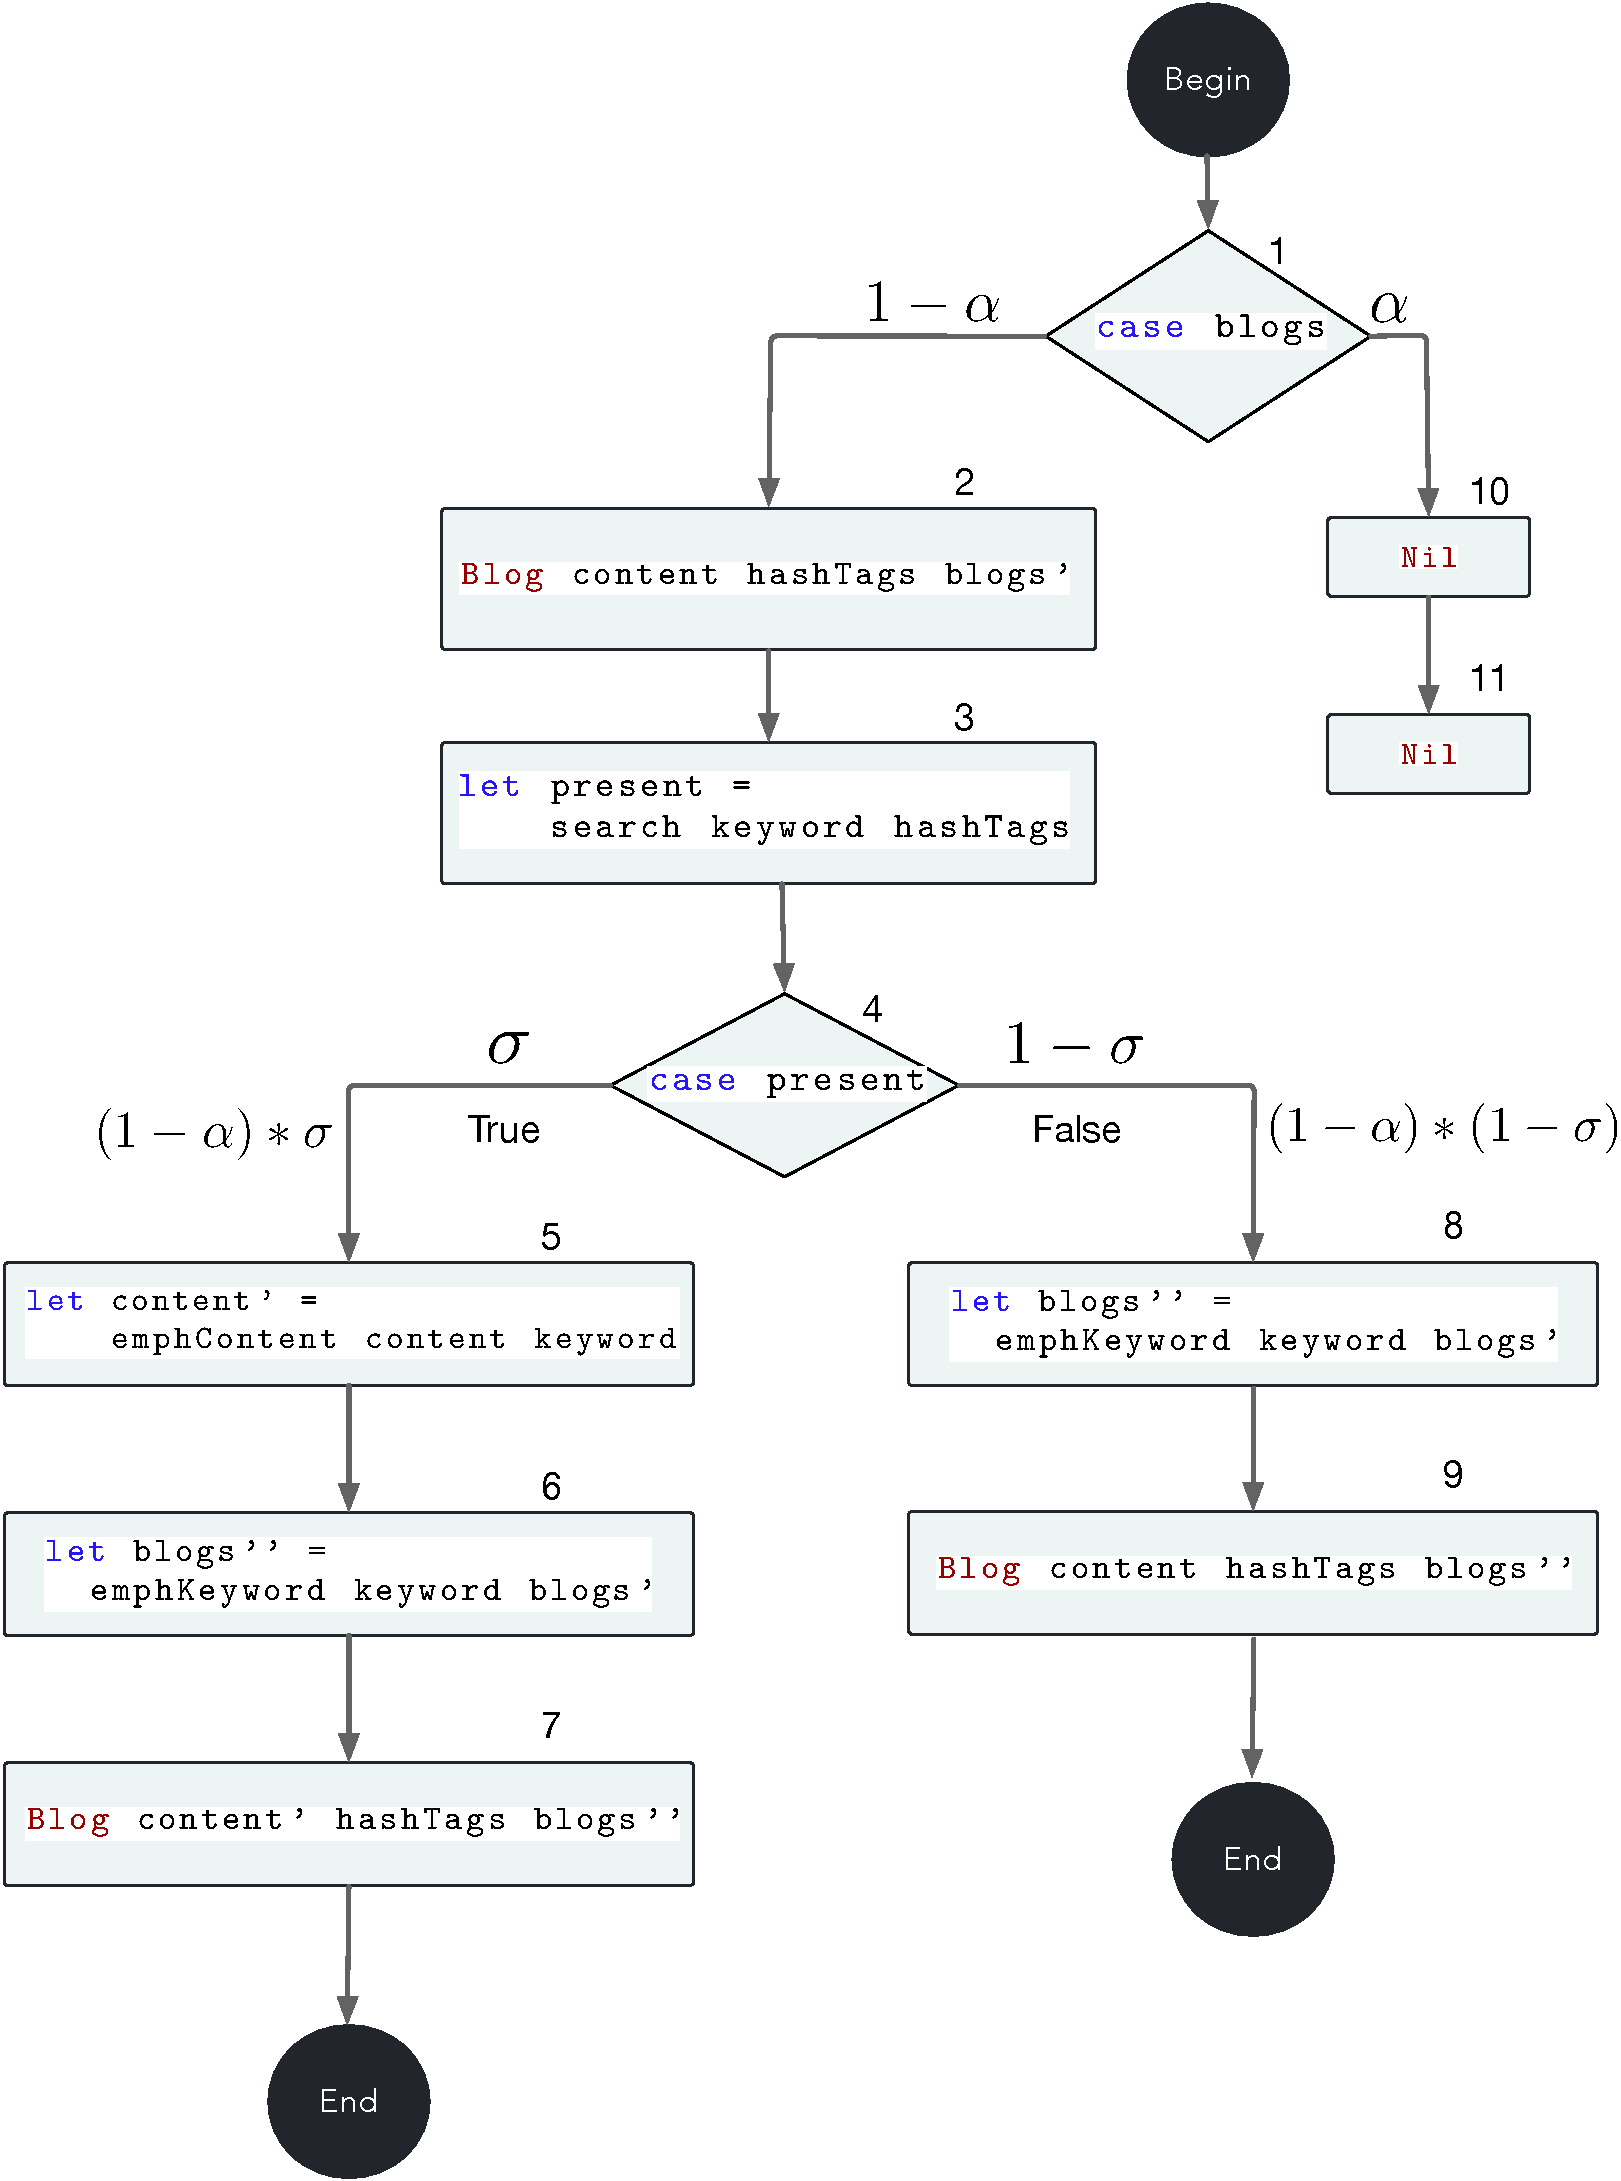
\includegraphics[scale=0.34]{figures/runningCFG}
  \caption{CFG with probability of executing along each path.}
  \label{graph:running-cfg}
\end{subfigure}
\begin{subfigure}[]{0.29\textwidth}
    \centering
  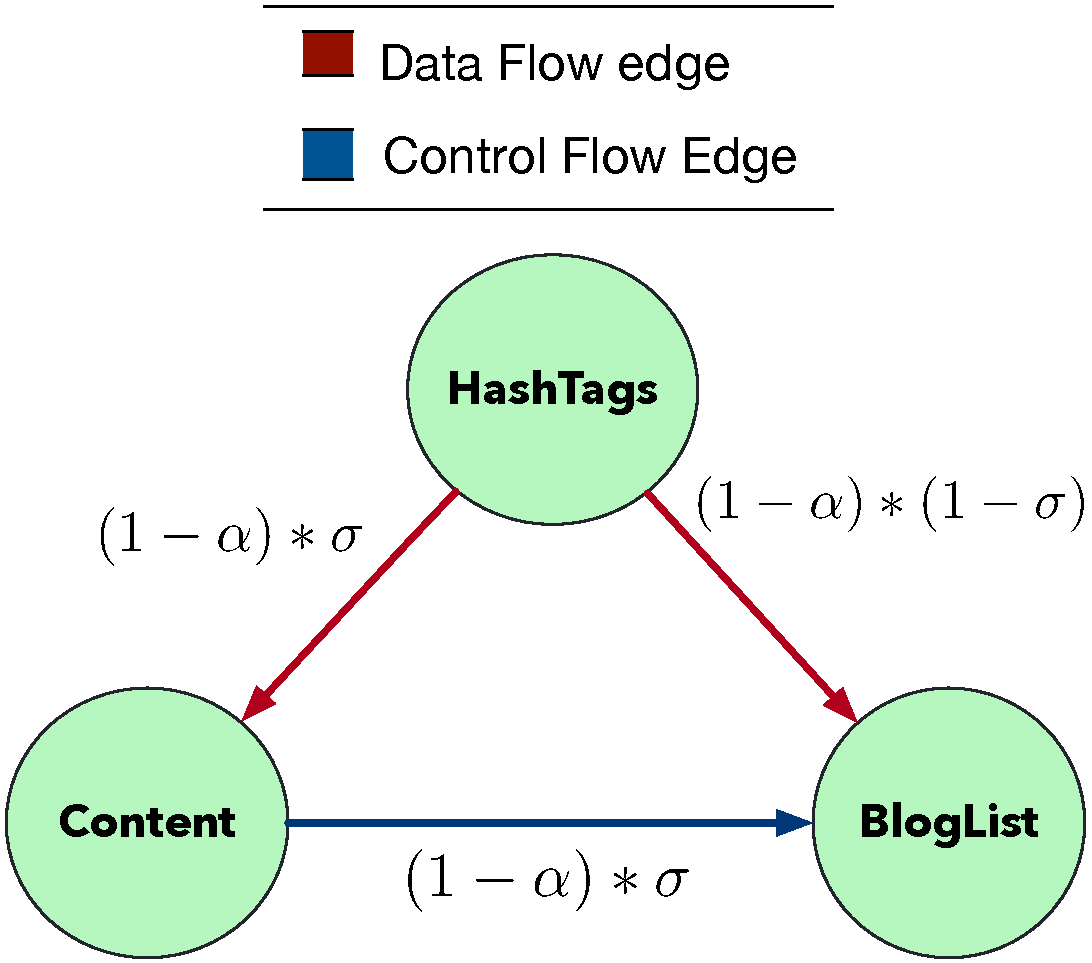
\includegraphics[scale=0.20]{figures/access-graph-running}
  \caption{Field-access graph $G$ generated from control-flow graph.
     Here we use field types to uniquely name them, since Haskell 
     record syntax was not used in this example to give each field a name.}
  \label{graph:running-access}
\end{subfigure}
\caption{Control-flow and corresponding field access graphs generated for the running example.}
\end{figure}
%\ap{TODO: the graphs go on the margins -- we should fix it. E.g. there is space now to put them back side by side}}


\subsection{Data Flow Analysis}
\label{design:dfa}

%\vs{Section Goal: Define why we need the data flow analysis and a quick summary of how we do it in the compiler.}

We implement a straightforward analysis (use-def chain, and def-use chain) for \lstinline|let| expressions to capture dependencies between 
\lstinline|let| expressions. We use this dependence information to form dataflow edges in the field access graph (\secref{design:fieldgraph})
and to subsequently optimize the layout and code of the traversal for performance. For \textit{independent} \lstinline|let| expressions in the function we are optimizing, we can transform the function body to have these let expressions in a different order. 
(Independent implies that there are no data dependencies between such \lstinline|let| expressions. Changing the order of independent \lstinline|let| expressions will
not affect the correctness of
% [non-crashing]
code, modulo exceptions.)
%\rn{Nontermination should be the same irrespective of let-binding order... we could swap nontermination and a panic as long as we have a partial language though... we reserve the right to do that?}
%
However, we do such a transformation only when we deem it to be more cost efficient. In order to determine 
when re-ordering \lstinline|let| expressions is more cost efficient, we classify fields based on specific attributes next.

\subsection{Field Attributes For Code Motion}
\label{subsec:attributes}

%% \vs{Section Goal: what are these attributes and how will they help getting a lost cost ordering. }

When trying to find the best layout, we may treat the code as immutable,
but allowing ourselves to move the code around (i.e. change the order of accesses to the fields)
unlocks more possibilities for optimizing layout.
Not all code motions are valid due to data dependencies in the traversal.
For instance, in a sequence of two \lstinline|let| binders, the second one may reference the binding introduced in the first one: in this case, the two binders cannot be reordered.

To decide which code motions are allowed, we classify each field with one or more of the attributes: \textit{recursive, scalar, self-recursive}, or \textit{inlineable}.
%
% Artem: the following needs a separate paragraph
% As there is a dependence between attributes, it may be possible to inherit multiple sub-attributes from a single attribute.
Some of these attributes are derived from the ADT definition and some from the code using the ADT.
%
A \emph{scalar} field refers to a datatype only made up of either other primitive types, such as \lstinline|Int|.
%
A \emph{recursive} field refers to a datatype defined recursively.
%the values constituting the field contain one or more recursive fields.
% \rn{Reword this --- fields have a type, but fields don't directly consist of other fields so this sounds a bit odd.}
%
A \emph{self-recursive} field is a recursive field that directly refers back to the datatype being defined (such as a \lstinline|List| directly referencing itself).
% similar to recursive fields but they are self-recursive since they contain fields that are the same type 
%% for instance the \lstinline|List| data type 
%% \begin{lstlisting}
%% data List = Nil | Cons Int List
%% \end{lstlisting}
%% Here \lstinline|List| is a recursive and a self-recursive field.
% \textit{Inlineable fields:}
Finally, we call a field \emph{inlineable} if the function being optimized makes a recursive call into this field \new{(i.e.\ taking the field value as an argument)}.
Hence, an inlineable field is necessarily a recursive field.
As we show in the example below, the inlineable attribute is especially important when choosing whether or not to do code motion.
%A field has this attribute based on the scope (that is, how it is used in a function.)
%In the running example, the \lstinline|BlogList| field is an inlineable field.

% For each function in the program, we introduce a new metadata field that stores the \new{attributes for all fields of all data constrcuctors used in that function.}
%% , for each data constructor, a mapping from each field index to all the possible attributes we can deduce about that particular field.
%
A single field can have multiple attributes.
For instance, a function \lstinline|traverse| doing a pre-order traversal on a \lstinline|Tree| makes recursive calls on both the
left and right children. The left and right children are recursive and self-recursive. Therefore, when looking at the scope of 
traverse, the left and right children have the attributes recursive, self-recursive and inlineable. 
%\vs Trying to talk about why having such attributes is helpful}

% Table to show the performance difference between List and List' 
% \ifx\ExtendedVersion\undefined
% \else
\begin{table}[t]
    \centering
    \caption{Running times for two traversals working with their corresponding matching layouts.}
    \begin{tabular}{ccc}
    \toprule
    datatype / traversal & \lstinline|List| / \lstinline|foo| & \lstinline|List'| / \lstinline|foo'| \\
    \midrule
    {1M elements} & 0.992s & 0.953s \\
    \bottomrule
    \end{tabular}
    \label{table:list-power}
\end{table}
%\fi

\begin{figure}[]
\centering
\begin{subfigure}{.5\textwidth}
    \centering
\begin{lstlisting}
  foo :: List -> List
  foo lst = case lst of
   Nil -> Nil
   Cons x rst ->
     let x' = x ^ 100
         rst' = foo rst
      in Cons x' rst'
\end{lstlisting}
\caption{Function \lstinline|foo| with \lstinline|List|.}
\label{fig:foo}
\end{subfigure}%
\begin{subfigure}{.5\textwidth}
    \centering
\begin{lstlisting}
  foo' :: List' -> List'
  foo' lst = case lst of
   Nil' -> Nil'
   Cons' rst x ->
     let rst' = foo' rst
         x' = x ^ 100
      in Cons' rst' x'
\end{lstlisting}
\caption{Function \lstinline|foo'| with \lstinline|List'|.}
\label{fig:foo'}
\end{subfigure}
\caption{Two different traversals on a list.}
\label{fig:two-diff-traversals}
\end{figure}

\textbf{Example.}
Consider the example of a list traversal shown in Figure~\ref{fig:foo}.
%
%We modify the \lstinline|List| type to contain a recursive field rather than an \lstinline|Int| to show an appreciable performance difference. 
%However, the core idea would be the same if the field were to be an \lstinline|Int| instead. 
%
%
%
Here the function \lstinline|foo| does some work on the \lstinline|Int| field (it raises the \lstinline|Int| to the power of 100) and then recurs on the tail of the list.
%
Since \system compiles to dense representations, a \lstinline|List|'s representation
in memory stores the \lstinline|Cons| tag (one byte) followed by the \lstinline|Int| (8 bytes) followed by
the next \lstinline|Cons| tag and so on. Hence, the \lstinline|Cons| tag and the \lstinline|Int| field are interleaved together in memory.
%
The function \lstinline|foo| becomes a stream processor that consumes one stream in memory and produces a dense output buffer of the same type.

Alternatively, another layout of a list follows from the following definition:
\begin{lstlisting}
  data List' = Nil' | Cons' List' Int
\end{lstlisting}
%
In memory, the list has all \lstinline|Cons'| tags next to each other \new{(a unary encoding of array length!)} and the \lstinline|Int| elements all next to each other.
%
In such a scenario, the performance of our traversal \lstinline|foo| on the \lstinline|List'| can improve 
% is a function of the work per element done and the size of the element field.
% 
%% As the work done on the element field increases or the length of the 
%% field itself increases, the cost to traverse the field reduces in the second representation because fields are packed next to each other.
traversal performance due to locality when accessing elements stored side-by-side\footnote{However, this effect can disappear if the elements are very large or the amount of work done per element becomes high, such that the percent of time loading the data is amortized.}.
%
However, this only works if we
can subsequently change the function that traverses the list to do recursion on the tail of the list first and then call the exponentiation
function on the \lstinline|Int| field after the recursive call. If there are no data dependencies between the recursive call and the exponentiation
function, then this is straightforward. We show \lstinline|foo'| with the required code motion transformation to function \lstinline|foo| accompanied
with the change in the data representation from \lstinline|List| to \lstinline|List'| as shown in Figure~\ref{fig:foo'}.

%% \rn{We also kill tail recursion! I don't think we can let that go by without mention... Our new function must have available stack space equal to list length. The original ``foo'' isn't tail recursive in the original sense either, but Gibbon can make it so because of how the prefix of the data constructor can be written BEFORE the recursion.}	     


				
% Consider the code snipped below, where we unroll the list and the recursive call to show what Inlining the recursive call looks like. Here we unroll the list to length 3 and call doWork 3 times. Although we have inlined the recursion, the data represenation is still interleaved, that is, the Integers are not packed next to each other as nicely as they would be in the List' representation of the List.
% With the foo' and List' representation, we are making all the recusive calls and then doing work on the Integers, albeit in the reverse order, However this still results in a friendlier memory access and runtime performance.

% \begin{lstlisting}
% foo :: List -> List 
% foo lst = case lst of 
% 	Nil -> Nil 
% 	Cons1 r1 Cons2 r2 Cons3 r3 ... rst -> 
% 	 let r1' = doWork r1 
% 	     r2' = doWork r2 
% 	     r3' = doWork r3 
%          .... 
%          rst ' = foo rst
%        in Cons r1' Cons r2' Cons r3' ... rst' 
% \end{lstlisting}

To optimize the layout, the tail of the list is assigned the attribute of inlineable. This attribute is used by the solver to
determine a least-cost ordering to the \lstinline|List| datatype in the scope of function \lstinline|foo|. 
Whenever such code motion is possible, \system will place the inlineable field first and use code-motion to change
the body of the function to perform recursion first if data flow dependencies allow such a transformation. 

% \ifx\ExtendedVersion\undefined
%\else
In fact, we made a similar program and ran \system on the program in the hope that it would be able to optimize the program by placing the inlineable
field first and use code-motion to change the traversal. We show the results in table~\ref{table:list-power}. We see a speedup of 4.1\% 
over our baseline datatype and traversal.
%\fi

\textbf{Structure of arrays.}
The transformation of
\lstinline|List|/\lstinline|foo| to \lstinline|List'|/\lstinline|foo'|
is similar to
%inlining the recursive call and
changing the representation of the \lstinline|List| datatype to a
\textit{structure of arrays}, which causes the same types of values to be next to each other in memory.
In particular, we switch from alternating constructor tags and integer values in memory to
an array of constructor tags followed by an array of integers.

Note that the traversals \lstinline|foo| and \lstinline|foo'| have access
patterns that are completely aligned with the data layout of \lstinline|List| and \lstinline|List'| respectively. The resulting speedup 
is solely a consequence of the \textit{structure of arrays} effect. This is an added benefit to the runtime in addition to ensuring that the 
access patterns of a traversal are aligned with the data layout of the datatype it traverses.

% Artem: we already considered the simpler example of List. Let's do the Blog example if we have space

% In the traversal from figure~\ref{fig:blog-traversal},
% the \lstinline|HashTags| field induces a data dependence through the \lstinline|if| statement caused by the call
% to \lstinline|search|. For that reason, we cannot change the code that causes the access to the \lstinline|HashTags|
% field. However, in the \lstinline|then| branch, the let expressions that cause the access to the content and tail of
% the list are not bound by any data dependence. We cannot move them out of the \lstinline|then| branch because of the
% data dependence from \lstinline|HashTags|, however, within the \lstinline|then| branch we can re-order the let expressions
% that access the content and the tail of the list respectively.

% For the running \lstinline|Blog| example, \system chooses
% a layout where \lstinline|HashTags| is followed by the tail pointer \lstinline|BlogList| and \lstinline|Content| respectively.
% \begin{lstlisting}
%     data BlogList = Nil | Blog HashTags BlogList Content
% \end{lstlisting}
% The traversal also changes such that the recursive call to the tail of the list \lstinline|BlogList| occurs first, followed by the call to emphasize
% the \lstinline|Content| in the \lstinline|then| branch. This layout and traversal transformation provides the best performance.

\subsection{Field Access Pattern Analysis}
\label{design:fieldgraph}

\begin{algorithm}[t]
        \caption{Recursive function for generating the field access graph}\label{alg:field-access-graph}
        \begin{algorithmic}[1]
            \small
            \Input
                \State cur: current CFG node from which to start processing
                \State dcon: data constructor for which we are searching the best layout
                \State edges: field-access graph built so far
                \State lastAccessedVar: last accessed variable name, initially None
                \State dfgMap: set of data-flow edges between variables
            \EndInput
            \Output
                \State Field access graph represented as a list of edges
                % \State \lsstinline|data Edge| = \lstinline|DfgEdge| ((var:\lstinline|String|, var:\lstinline|String|), likelihood:\lstinline|Int|)
                % \State             | \lstinline|CfgEdge| ((var:\lstinline|String|, var:\lstinline|String|), likelihood:\lstinline|Int|)
            \EndOutput
            \Function{FieldAccessGraph}{cur, dcon, edges, lastAccessedVar, dfgMap}

                \algorithmiclet{((expr, weight), successors) = cur} \label{line-likelihood-example}
                %\algorithmicletmutable{isFirstAccess = true}
                \algorithmicletmutable{lastAccessedVarMut = lastAccessedVar}
				\algorithmicletmutable{edges\textquotesingle = edges}
                \For{var : \Call{OrderedFreeVariables}{expr}} \label{line:lastAccessedVar-start}
                    \If{!\Call{BoundInPatternMatchOnDcon}{var, dcon}} \label{line:boundInDcon}
						\Continue
					\EndIf
                        \If{lastAccessedVarMut != None}
							\algorithmicmutate{edges\textquotesingle = \Call{addEdge}{edges\textquotesingle, ((lastAccessedVar, var), weight), ControlFlowTag}}\label{line:cfg-edge}
                            \If{\Call{lookup}{(lastAccessedVar, var), dfgMap}}
                                \algorithmicmutate{edges\textquotesingle = \Call{addEdge}{edges\textquotesingle, ((lastAccessedVar, var), weight), DataFlowTag}}\label{line:dfg-edge}
                            \EndIf
                        \EndIf
                        \algorithmicmutate{lastAccessedVarMut = var}
                \EndFor \label{line:lastAccessedVar-end}
                
                \For{succ : successors} \label{line:succ-rec-start}
                    \algorithmiclet{edges\textquotesingle\textquotesingle = \Call{FieldAccessGraph}{succ, dcon, edges\textquotesingle, lastAccessedVarMut, dfgMap}}
                    \algorithmicmutate{edges\textquotesingle = \Call{merge}{edges\textquotesingle, edges\textquotesingle\textquotesingle}}
                \EndFor \label{line:succ-rec-end}

                \State \Return edges\textquotesingle

            \EndFunction

            % \Function{AccessGraphDriver}{cfgMap, dfgMap, functions}
                
            %     \State letMutable accessGraphMap = newEmptyMap
            %     \For{funcName : functions}
            %         \State let dconsInFunc = \Call{getDataConstructors}{funcName}
            %         \State let funcCfg = \Call{Map.lookup}{cfgMap, funcName}
            %         \State let cfgRoot = \Call{getCfgRoot}{funcCfg}
            %         \State let funcDfg = \Call{Map.lookup}{dfgMap, funcName}
            %         \For{dcon : dconsInFunc}
            %             \State let edges = \Call{AccessGraph}{None, cfgRoot, dcon, [], None, funcDfg}
            %             \State \Call{Map.insert}{accessGraphMap, (funcName, dcon), edges}
            %         \EndFor
            %     \EndFor
            %     \State \Return accessGraphMap
            % \EndFunction

            % \Function{AddEdge}{edgeList, edge}
            %     \State let reversedEdge = \Call{reversedAccessEdge}{edge}
            %     \If{!\Call{exists}{reversedEdge, edgeList}}
            %         \State \Call{append}{edgeList, edge}
            %     \EndIf
            % \EndFunction
        \end{algorithmic}
    \end{algorithm}


After constructing the \CFG and \DFG for a function definition, we utilize them to inspect the type
of each of the function's input parameters---one data constructor at a time---and construct
a \emph{field-access graph} for it.
Algorithm~\ref{alg:field-access-graph} shows the psuedocode for generating the field-access graph. 
%
This graph represents the temporal ordering of accesses among its fields.

The fields of the data constructor form the nodes of this graph.
%
A directed edge from field $f_i$ to field $f_j$ is added if $f_i$ is accessed immediately before $f_j$. Lines~\ref{line:lastAccessedVar-start} to ~\ref{line:lastAccessedVar-end}
in Algorithm~\ref{alg:field-access-graph} show how we keep track of the last accessed field and form an edge if possible. 
A directed edge can be of two different types. In addition, each edge has a associated weight which indicates the likelihood of accessing $f_i$ before $f_j$, which is computed using the \CFG.
An edge can either be a data-flow edge or a control-flow edge (Lines~\ref{line:cfg-edge} and ~\ref{line:dfg-edge}). In \Figref{graph:running-access}, the red edge is a data flow edge and the blue edge is a control flow edge.

\textit{Data-Flow Edge} indicates an access resulting from a data flow dependence between the fields $f_i$ and $f_j$. In our source language, a data flow edge is induced by
% either an \lstinline|if| conditional or
a \lstinline|case| expression.
A data flow edge implies that the code that represents the access is rigid in structure and changing it can make our transformation invalid.

\textit{Control-Flow Edge} indicates an access that is not data-flow dependent. It is caused by the control flow of the program. Such an edge does not induce strict constraints on the code that induces the edge. The code is malleable in case of such accesses. This gives way to an optimization search space via code motion of \lstinline|let| expressions. The optimization search space involves transformation of the source code, i.e, changing the access patterns at the source code level.
%The transformation is possible because there is no data dependence that prevents changing the order of access between the fields. 
%
%% %
%% Branching in the \CFG leads to three possible scenarios of field accesses:
%% \begin{itemize}
%% \item todo.
%% \end{itemize}

%% \csk{stopped writing here.}

%% Loosely similar to Chilimbi~\etal~\cite{CSD, CSL, ccgarbage} we construct what we formally call a \textit{field access} graph (subsequently referred to as $G$) that captures the static temporal access patterns of the fields for a particular data constructor. Hence, in our current model, we store such a $G$ for a unique quadruple $(\PROG, \FD, \DD, \sDC)$. The graph $G(V, E)$ is a weighted directed graph where each vertex  $v \epsilon V$ is a field($\fields$) from the fields($\vectorize{\fields}$) of a data constructor($\sDC$). Each edge $e \epsilon E$ represents an access between two fields.

%% For now, we locally optimize the ordering of the fields ($\vectorize{\fields}$) of a data constructor $\sDC$ for a packed type $\DD$. The objective of the ordering problem is to match the data layout of each data constructor $\sDC$, that is, the layout of all fields $\vectorize{\fields} \epsilon \sDC$ to the
%% access patterns of the traversal $\FD$ operating on the fields of the data constructor.

%% To be able to match the data layout of a value constructor $\sDC$ in memory to the traversal order of the function whose performance we are optimizing (Such a function and the corresponding data type to be optimized is annotated by the user while writing the top level program) we need to have information about the temporal access patterns of each field in the data constructor.

%% There have been prior works that solve a similar problem~\cite{CSD, CSL, ccgarbage} but they are designed to work with imperative programming languages like \textit{C and C++}. In addition, the problem there is concerned with optimizing the memory layout of boxed data structures that are not statically and readily packed in memory like with \system.
 
The field-access graph $G$ is a directed graph, which consists of edges of the two types between fields of a datatype and can have cycles. The directed nature of the edges enforces a temporal relation between the corresponding fields. More concretely, assume that an edge $e$ that connects two vertices representing fields $\fields_{a}$ (source of $e$) and $\fields_{b}$ (target of $e$). We interpret $e$ as an evidence that field $\fields_{a}$ is accessed before field $\fields_{b}$. The weight $w$ for the edge $e$ is the probability that this access will happen based on statically analyzing a function. % $\FD$.

In our analysis, for a unique path through the traversal, we only account for the {\em first} access to any two fields. If two fields are accessed in a different order later on, the assumption is that the start address of the fields is likely to be in cache and hence it does not incur an expensive fetch call to memory. In fact, we tested our hypothesis by artificially making an example where say field $f_{a}$ is accessed first, field $f_{b}$ is accessed after $f_{a}$ after which we constructed multiple artificial access edges from $f_{b}$ to $f_{a}$, which might seem to suggest placing $f_{b}$ before $f_{a}$. However, once the cache got warmed up and the start addresses of $f_{a}$ and $f_{b}$ are already in cache, the layout did not matter as much. This suggests that prioritizing for the first access edge between two unique fields along a unique path is sufficient for our analysis.

Two fields can be accessed in a different order along different paths through a traversal. This results in two edges between the fields. (The edges are in reversed order.) We allow at most two edges between any two vertices with the constraint that they have to be in the opposite direction and come from different paths in the traversal. If two fields are accessed in the same order along different paths in the traversal, we simply add the probabilities and merge the edges since they are in the same direction.

In order to construct $G$, we topologically sort the control-flow graph of a function %$\FD$
and traverse it in the depth-first fashion via recursion on the successors of the current cfg node (Lines~\ref{line:succ-rec-start} to~\ref{line:succ-rec-end}).
%
As shown in line~\ref{line:boundInDcon}, we check if a variable is an alias to a field in the data
constructor for which we are constructing the field-access graph $G$.
%
As we process each node (i.e. a primitive expression such as a single
function call), we update the graph for any direct or indirect
references to input fields that we can detect.
%
We ignore new variable bindings that refer to newly allocated rather
than input data---they are not tracked in the access graph.
%
%% For the current node being processed in the control flow graph, ,
%% % i.e, instruction,
%% we back track each input variable to figure out if it is an alias to
%
%% Since we are in a functional programming paradigm, we restrict this
%% analysis for variables introduced in a \textit{case} binding or
%% function arguments since we assume that variables that are written
%% to are allocated in a fresh memory location. Hence, accesses to
%% newly written fields do not optimize the in memory layout of the
%% data constructor that is being read and is input to the traversal.
%
\auditme{We traverse the control-flow graph once, but we maintain the
  last-accessed information at each CFG node, so when we process a field
  access at an expression, we consult what was previously-accessed at
  the unique precedecessor of the current CFG node.}
%
\Figref{graph:running-access} shows the generated access graph from the control-flow graph in \figref{graph:running-cfg}. It also shows the probability along each edge obtained from the control-flow graph.

%% For each such variable which originates from one of the fields of the data constructor in scope, we traverse all the successor nodes in the control flow graph to see is there are any other fields that are accessed in the successor nodes. For the fields that are accessed, we add a directed edge from the current field to the successor field/s. We recursively do this for all the successors and terminate when we have completely traversed the graph in topological order.
%% \rn{This makes it sound like we do a bunch of repeated traversals -- traversing the downstream graph every time we have an access.}

As we are traversing the nodes of the control-flow graph and generating directed edges in $G$, we use the likelihood of accessing that cfg node as the weight parameter (Line~\ref{line-likelihood-example}).
%As mentioned previously, we can get more precise weights by dynamically profiling the traversal at runtime to obtain the frequency of taking a particular path through the traversal.
%However, for now, we restrict ourselves to static weights.

% \begin{figure}[]
%   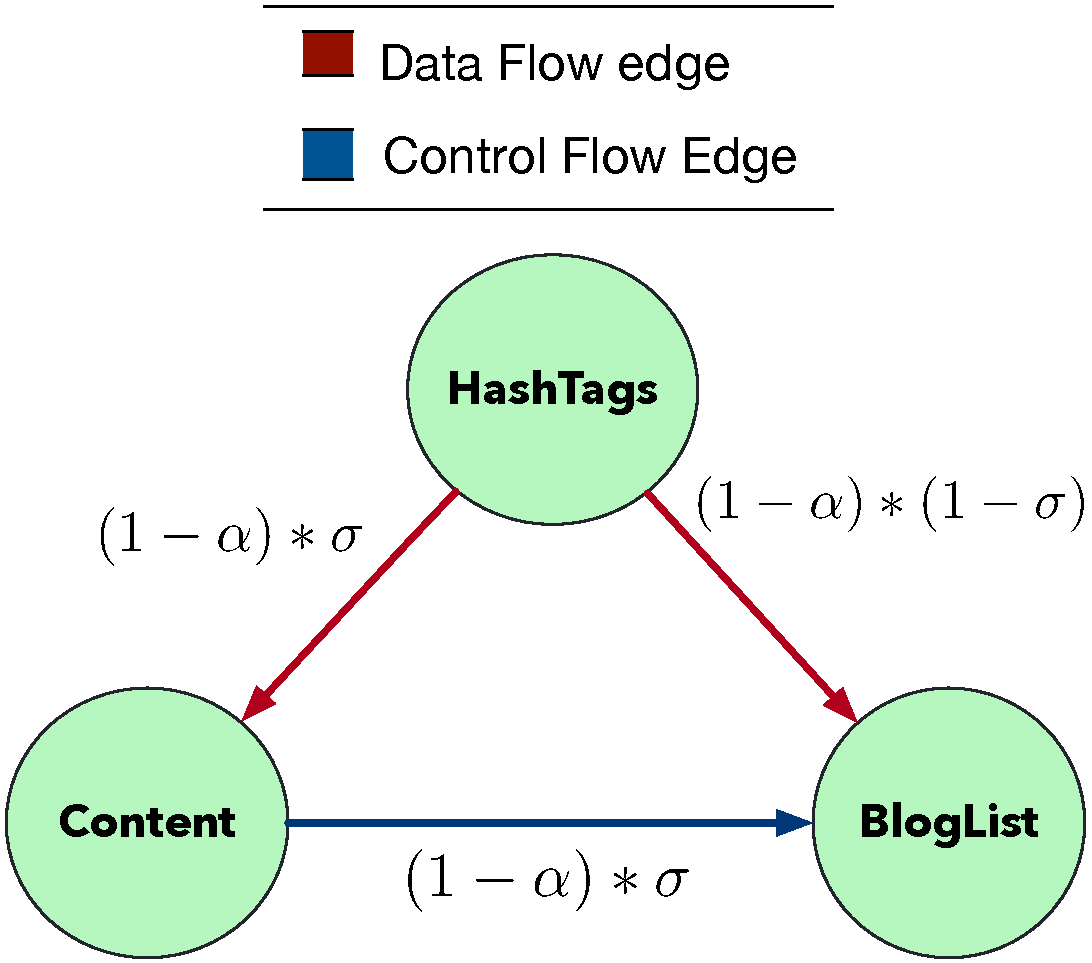
\includegraphics[scale=0.45]{figures/access-graph-running}
%   \caption{Field access graph $G$ generated from \CFG of running
%     example~\ref{graph:running-cfg}.  Here we use field types to
%     uniquely name them, since Haskell record syntax was not used in
%     this example to give each field a name.}
%   \label{graph:running-access}
% \end{figure}

\subsection{Finding a Layout}
\label{design:genconstraints}

%% \vs{Goal: define how the constraints are generated from the access pattern graph. That is, the cost model and all its components.}

% \rn{This paragraph was pretty repetitive:}
%% The field access graph for a value constructor in the ADT captures the access patterns of the fields in the value constructor by statically analyzing the traversal $\FD$ that consumes the ADT. The access paths of the fields induce concrete edges in the access pattern graph $G$. These edges are directed in nature and hence signify a temporal access pattern between the fields making up the edge. Each edge in the access pattern graph has an associated weight which is calculated statically for now.

We use the field-access graph $G$ to encode the problem of finding a better layout as an Integer Linear Program (ILP). Solving the problem yields a cost-optimal field order for the given pair of a data constructor and a function.

\subsubsection{ILP Constraints}
In our encoding, each field in the data constructor is represented by a variable, $f_0, f_1, \dots$ As a part of the result, each variable will be assigned a unique integer in the interval $[0, n -1]$, where $n$ is the number of fields. Intuitively, each variable represents an index in the sequence of fields.

The ILP uses several forms of constraints, including two forms of \emph{hard} constraints:
%
\begin{gather}
  \forall_{0 \leq i < n}  \qquad 0 \leqslant f_{i}  < n \label{eq:valid}\\
  \forall_{0 \leq i < j < n} \qquad f_i \neq f_j   \label{eq:uniq}
\end{gather}
%
The constraints of form~\ref{eq:valid} ensure that each field is mapped to a valid index, while the constraints of form~\ref{eq:uniq} ensure that each field has a unique index.
Constraints of either form must hold because each field must be in a valid location.

Hard constraints define valid field orderings but not all such reorderings improve efficiency, \system's main goal.
%
To fulfil the goal, beside the hard constraints we introduce {\em soft} ones. Soft constraints come from the field access analysis. For example, assume that based on the access pattern of a function, we would {\em prefer} that field $a$ goes before field $b$. We turn such a wish into a constraint. If the constraint cannot be satisfied, it will not break the correctness. In other words, such constraints can be broken, and that is why we call them soft.

\subsubsection{Cost Model}
\system encodes these soft constraints in the form of an abstract cost model that assigns a cost to a given layout (assignment of fields to positions) based on how efficient it is expected to be given the field-access graph.

To understand the intuition behind the cost model, note that the existence of an edge from field $f_i$ to field $f_j$ in the field-access graph means that there exists at least one path in the control-flow graph where $f_i$ is accessed and $f_j$ is the next field of the data constructor that is accessed.
%
In other words, the existence of such an edge implies a preference {\em for that control-flow path} for field $f_i$ to be immediately before field $f_j$ in the layout so that the program can continue a linear scan through the packed buffer.
%
Failing that, it would be preferable for $f_j$ to be ``ahead'' of $f_i$ in the layout so the program does not have to backtrack in the buffer.
%
We can thus consider the costs of the different layout possibilities of $f_i$ and $f_j$:

\begin{description}
	\item[$C_{\mathit{succ}}$] ($f_j$ immediately after $f_i$): This is the best case scenario: the program traverses $f_i$ and then uses $f_j$.
	\item[$C_{\mathit{after}}$] ($f_j$ after $f_i$ in the buffer): If $f_j$ is after $f_i$, but not {\em immediately} after, then the code can proceed without backtracking through the buffer, but the intervening data means that either a shortcut pointer or a \new{extra traversal} must be used to reach $f_j$, adding overhead.
	\item[$C_{\mathit{pred}}$] ($f_j$ immediately before $f_i$): Here, $f_j$ is {\em earlier} than $f_i$ in the buffer. Thus, the program will have already skipped past $f_j$, and some backtracking will be necessary to reach it. This incurs {\em two} sources of overhead: skipping past $f_j$ in the first place, and then backtracking to reach it again.
	\item[$C_{\mathit{before}}$] ($f_j$ before $f_i$ in the buffer): If, instead, $f_j$ is farther back in the buffer than $f_i$, then the cost of skipping back and forth is greater: in addition to the costs of pointer dereferencing, because the fields are far apart in the buffer, it is less likely $f_j$ will have remained in cache (due to poorer spatial locality).
\end{description}

We note a few things. 
%
First, the {\em exact} values of each of these costs are hard to predict. 
%
The exact penalty a program would pay for jumping ahead or backtracking depends on a variety of factors such as cache sizes, number of registers, cache line sizes, etc.
%
%Second, one could imagine a more fine-grained cost model that distinguishes between, say, fields that are a constant distance apart versus those that have some other recursive (and hence potentially large) field between them.
%
%However, the inexact nature of the cost model means that this would be false precision.
%
%Instead, \system uses an abstract cost model with reasonably-chosen values satisfying the following:

However, we use our best intuition to statically predict these costs based on the previously generated access graph.
Note the existence of two types of edges in our access graph. An edge can either be a data-flow edge or a control-flow edge.
For a data flow edge, the code is rigid. Hence the only axis we have available for transformation is the datatype itself. For a data flow edge, the costs are showed in Eq~\ref{eq:costs-strong-edge}. Here, we must respect the access patterns in the original code which lead to the costs in Eq~\ref{eq:costs-strong-edge}.
%
\begin{equation}
C_{\mathit{succ}} < C_\mathit{after} < C_\mathit{pred} < C_\mathit{before}
\label{eq:costs-strong-edge}
\end{equation}

Note that a control-flow edge signifies that the direction of access for an edge is transformable. We could reverse the access in the code without breaking the correctness of the code. We need to make a more \textit{fine-grained} choice.
This choice involves looking at the attributes of the fields and making a judgement about the costs given we know the attributes of the fields. As shown in Sec~\ref{subsec:attributes} we would like to have the field with an \textit{inlineable} attribute placed first.
Hence, in our cost model, if $f_i$ is inlineable, then we follow the same costs in Eq~\ref{eq:costs-strong-edge}. However, if $f_j$ is inlineable and $f_i$ is not, we would like $f_j$ to be placed before $f_i$. For such a layout to endure, the costs should change to Eq~\ref{eq:costs-inlineable}.
For other permutations of the attributes, we use costs that prioritize placing the inlineable field/s first. 
\begin{equation}
C_\mathit{pred} < C_\mathit{before} < C_{\mathit{succ}} < C_\mathit{after}
\label{eq:costs-inlineable}
\end{equation}


\subsubsection{Assigning Costs to Edges}

\system uses the field-access graph and the cost model to construct an objective function for the ILP problem.
%
Each edge in the access graph represents one pair of field accesses with a preferred order. Thus, for each edge $e = (i, j)$, \system can use the indices of the fields $f_i$ and $f_j$ to assign a cost, $c_e$, to that pair of accesses following the rules below.
\begin{table}[h]
\centering
\begin{tabular}{ll}
If $f_j$ is right after $f_i$, then assign cost $C_\mathit{succ}$, i.e.:
&
$
(f_j - f_i) = \phantom{-}1 \implies c_e = C_\mathit{succ}
$.
\\
%
If $f_j$ is farther ahead of $f_i$, then assign cost $C_\mathit{after}$, i.e.:
&
$
(f_j - f_i) > \phantom{-}1 \implies c_e = C_\mathit{after}
$.
\\
%
If $f_j$ is immediately {\em before} $f_i$, then assign cost $C_\mathit{pred}$, i.e.:
&
$
(f_j - f_i) = -1 \implies c_e = C_\mathit{pred}
$.
\\
%
And if $f_j$ is farther before $f_i$, then assign cost $C_\mathit{before}$, i.e.:
&
$
(f_j - f_i) < -1 \implies c_e = C_\mathit{before}
$.
\end{tabular}
\end{table}

The cost of each edge, $c_e$ must be multiplied by the {\em likelihood} of that edge being exercised, $p_e$, which is also captured by edge weights in the field-access graph. Combining these gives us a total estimated cost for any particular field layout:
%
\begin{equation}
C = \sum_{e \in E} c_e \cdot p_e
\label{eq:objective}
\end{equation}
%
This is the cost that our ILP attempts to minimize, subject to the hard constraints~\ref{eq:valid} and~\ref{eq:uniq}.

\subsubsection{Greedy layout ordering}

\new{
Finding an optimal layout using an external solver hurts compile times.
To solve this tradeoff, we propose a simple algorithm that traverses the field access graph in a \emph{greedy} fashion.
The algorithm starts from the root node of the graph, which corresponds to the field accessed first in the function, and greedily visits the child nodes based on the edge weights.
}
We fix the edge order for a control-flow edge as the original order and do not look at field attributes. However, after the greedy algorithm picks a layout we match the let expressions to the layout order to make sure the code matches the layout order. The greedy algorithm is potentially sub-optimal when it comes to finding the best performing layout; however, the compile time is fast.

%Since there is a tradeoff in compile-times and run-times we wanted to ensure that we have a backend with a fast compile time in case compile time becomes a bottleneck.  

\subsection{Finding a global layout}
\label{design:global}

A data constructor can be used across multiple functions, therefore, we need to find a layout order that is optimal globally.
To do so, we take constraints for each function and data constructor pair and combine them uniformly, that is, a uniform weight for each function.
%\footnote{Dynamic profiling techniques can be used to get more precise weights, but we leave such efforts for future work.}.
We then feed the combined constraints to the solver to get a globally optimal layout for that data constructor. The global optimization finds a globally optimal layout for all data constructors in the program. Once the new global layout is chosen for a data constructor, we re-write the 
entire program such that each data constructor uses the optimized order of fields.
In the evaluation, we use the global optimization. However, we only show the data constructor that constitutes the major part of the program.

\subsection{Finding a layout for functions with conflicting access patterns}
\label{design:conflicting-access-patterns}
Consider the datatype definition \lstinline|D| with two fields \lstinline|A, B|:
\begin{lstlisting}
    data D = D A B
\end{lstlisting}
If two functions, \lstinline|f1| and \lstinline|f2|, access the fields of \lstinline|D| in the opposite orders,
we get conflicting access patterns for \lstinline|D|.
For instance, assume \lstinline|f1| accesses \lstinline|A| first and then \lstinline|B|, while \lstinline|f2|
accesses \lstinline|B| first and then \lstinline|A|. After combining edges across the two functions, we get two edges
in opposition to each other. Since we use uniform weights for all functions, the edges will also have a uniform weight.
As a result,
placing \lstinline|A| before \lstinline|B| or vice versa are equally good in our
cost model, and \system defers to the solver to get one of the two layouts.

\new{
With the two equally good layouts, \system's solver (the default mode) chooses the layout favoring the function it picked first. For instance, if \lstinline|f1| is defined earlier in the program, the order favoring \lstinline|f1| will be picked.
%
In the greedy mode, since both \lstinline|A| and \lstinline|B| are root nodes, \system will pick the
first root node in the list of root nodes, which is, again, dependent on the ordering of functions in the source code.
%
% If we determined that \lstinline|f2| has a greater weight than \lstinline|f1|, then the layout preferred by \lstinline|f2| would be chosen. % Artem: leaving hypoteticals to the discussion section
}

%Based on the relative positions of the two fields (in memory) making up an edge, the edge in the graph can take four different cost values
%% that we unfold in detail
%in our cost model.
%
%The objective of the ILP formulation is to minimize the sum of weighted costs for all the edges where the weight is the corresponding likelihood along each edge in the graph. 
%First we provide some definitions to describe our integer linear program. 
%
%\[ M = \text{The ILP model} \]
%\[ \sDC = \text{data constructor whose field order is being optimized} \]
%\[ n \equiv |\vectorize{\fields}| = \text{ total number of vertices in the graph G} \]
%\[ m = \text{ total number of edges in the graph G} \]
%\[ f_{1}, f_{2}, ... f_{n} \epsilon \vectorize{\fields}= \text{index variables for each field in $\sDC$} \]
%\[ c_{1}, c_{2}, ... c_{m} = \text{cost variables for edges }  e_{1}, e_{2} ... e_{m} \epsilon E \]
%\[ l_{1}, l_{2} ... l_{m} = \text{likelihood values for edges } e_{1}, e_{2} ... e_{m} \epsilon E \]
%
%\subsubsection*{Defining cost:}
% Let us assume the presence of a temporal access between two fields $f_1$ and $f_2$ in a function $\FD$ (assuming $f_1$ dominates $f_2$ in $G$). 
%Let us take a closer look at the time window when traversal $\FD$ has consumed field $f_1$ and is about to access field $f_2$. 
%
%There are two possibilities that can arise depending on how the fields $f_1$ and $f_2$ are laid out in the packed buffer. If field $f_2$ is serialized some fields after field $f_1$ {\em nonconsecutively}, then the traversal $\FD$ has to perform a \textit{forward pointer dereference} to get to field $f_2$.  On the other hand, if field $f_2$ is serialized before $f_1$ then the traversal has to \textit{backtrack} or do a \textit{backward jump} to get to field $f_2$.
%%
%\auditme{When moving forward, the size of the jump could be zero bytes (if the fields are consecutive), or an amount that depends on the size of what is skipped over (constant or variable).  Constant jumps are most efficient because they can be computed at compile time based on the ending byte of field $f_1$.}
%%
%%% \auditme{For the remainder of this paper we simply {\bf ignore fields with constant size (scalars)}. We leave them out of the analysis, and let the Gibbon compiler backend place them where it wants (which is currently directly after the tag byte identifying the data constructor).}
%\rn{TODO: make the above commented bit true...}
%
%In practice, for a forward pointer dereference, the packed representation provides the presence of a \textit{RAN} pointer (random access pointer or shortcut pointer) that the traversal can dereference to jump to the address $f_2$ is serialized at. For a backtrack, the traversal $\FD$ needs to know how to get to the start address of field $f_2$ in the packed buffer. This can be achieved by generating extra traversals over the packed buffer or storing the start address of $f_2$ as yet another \textit{RAN} pointer, \new{but the present Gibbon compiler infrastructure prefers the latter}.
%
%\begin{itemize}
%  \item \textit{forward pointer dereference:} The packed representation of the ADT provides the presence of a pointer which can be dereferenced to reach the location of the desired field we want to access. We store the cost of this pointer dereference as some \textit{p} in our model $M$.
%
%  \item \textit{backtrack or backward jump: } The function $\FD$ must rewind in the packed buffer to reach the start of the desired field. We store the cost of such a backward jump by function $\FD$ as \textit{b}. 
%\end{itemize}
%
%
%In our model $M$, we assign a cost for each edge $e$ based on the relative positions of fields $f_{i}$ and $f_{j}$. Let us assume this cost to be $c_{k}$; the cost $c_{k}$ can take four different values based on the relative positions of $f_{i}$ and $f_{j}$. These costs are constants known statically. These are derived based on the relative positions of the fields which induces a cost \textit{p} or \textit{b} or some combination of the two. These costs are shown below. The details of these costs are defined later on as we shall see. Currently in our model $M$, the costs \textit{p} and \textit{b} are assumed to be the same.
%
%\[ C_{1}, C_{2}, C_{3}, C_{4} \epsilon \mathbb{W} = \text{constant costs known statically, at compile time} \]
%
%\begin{equation}
%\centering
%C_{1} < C_{2} < C_{3} < C_{4}
%\tag{Cost relation}
%\label{eqn:constant-costs}
%\end{equation}
%
%Now that we have some definitions, we can generate some constraints for our model $M$. For an edge $e \epsilon E$ with an associated cost $c_{k}$ in the graph $G$, suppose fields $\fields_{i}$  and $\fields_{j}$ (represented by model variables $f_{i}$ and $f_{j}$ moving forward)  participate in that edge. Moreover, for the directed edge e, let $f_{i}$ dominate $f_{j}$ which implies that field $f_{i}$ is accessed prior to field $f_{j}$ along the path that goes through edge e in the graph $G$. We introduce four constraints (implications) for edge $e$ based on relative positions of $f_{i}$ and $f_{j}$ in the packed buffer. 
%
%The \textit{lhs} of the implication computes the difference of indices of the two fields (this emulates their relative position in memory) and the \textit{rhs} gives a cost based on the relative position. The following equations~\cref{eqn:imp1,eqn:imp2,eqn:imp3,eqn:imp4} define the constraints for an edge $e$ and we have these for each edge $e \epsilon E$.
%
%
%\begin{equation}
%\label{eqn:imp1}
%(f_{i} - f_{j}) =  -1  \Rightarrow (c_{k} = C_{1})      
%\tag{constr 1}
%\end{equation}
%
%\textit{If} fields $f_{i}$ and $f_{j}$ are right next to each other such that $f_{i}$ is to the left of field $f_{j}$ then such an arrangement induces an insignificant cost $C_{1}$ for the edge $e$. This is because the directed edge $e$ is interpreted as a temporal access from $f_{i}$ to $f_{j}$. A traversal that needs to access 
%$f_{i}$ right before $f_{j}$ would incur the least cost if $f_{i}$ was serialized right before $f_{j}$ in the packed buffer.
%
%\begin{equation}
%\label{eqn:imp2}
%(f_{i} - f_{j}) < -1  \Rightarrow (c_{k} = C_{2})  
%\tag{constr 2}
%\end{equation}
%
%\textit{If} field $f_{i}$ is to the left of $f_{j}$ and there are $t$ number of fields between them (where $t$ > 0) then the temporal access given by edge $e$ induces a cost $C_{2}$. The cost $C_{2}$ is greater that cost $C_{1}$ on account of the extra $t$ fields present between $f_{i}$ and $f_{j}$. In such a packed representation of the two fields, in order for a traversal to get from field $f_{i}$ to $f_{j}$ it needs to either forward jump or walk(using a dummy traversal) over the $t$ fields. This is the cost \textit{p} mentioned earlier. (in practice, \system provides a pointer to the starting address of field $f_{2}$)
%
%\begin{equation}
%\label{eqn:imp3}
%(f_{i} - f_{j}) =  1  \Rightarrow (c_{k} = C_{3})
%\tag{constr 3}
%\end{equation}
%
%\textit{If} fields $f_{i}$ and $f_{j}$ are right next to each other and $f_{i}$ is to the right of $f_{j}$ in the packed buffer, then, the edge $e$ induces a cost $C_{3}$ satisfying~\ref{eqn:constant-costs}.
%This cost is greater than $C_{1}$ and $C_{2}$. This is because in order for a traversal to first access $f_{i}$ in the packed buffer, it has to jump over the field $f_{j}$ serialized before it and then rewind (\textit{backtrack}) in the buffer to be able to access field $f_{j}$ again. This means that the traversal not only has to incur a cost of a forward pointer dereference but also incur an extra cost of a backtrack. Hence total cost is \textit{p + b}.
%
%\begin{equation}
%\label{eqn:imp4}  
%(f_{i} - f_{j}) >  1  \Rightarrow (c_{k} = C_{4})  
%\tag{constr 4}
%\end{equation}
%
%\textit{If} field $f_{i}$ is to the right of field $f_{j}$ and there are $t$ fields in between them in the packed representation (where $t$ > 0), then, the edge $e$ induces a cost $C_{4}$ which is the most expensive cost in our model $M$. Traversing such a packed buffer requires first a forward jump over $t$ fields to reach field $f_{i}$ and then backtrack to reach the start of field $f_{j}$. This is more costly than implication~\ref{eqn:imp3} since the traversal has to potentially jump across larger addresses in memory (especially if there is a recursive field in between). Such a jump will exhibit worse spatial locality. We can represent this cost as greater than implication~\ref{eqn:imp3} by multiplying it by a constant factor (i.e., \textit{c*(p + b)}, for some constant c). 
%
%
%The ILP model $M$ is a minimization problem where we solve for the optimal indices of the fields $\vectorize{\fields}$ such that it minimizes the total weighted costs along all the edges in the graph $G$. The weights are simply the likelihoods along each edge in the graph $G$ which are constants known statically.
%
%\begin{equation}
%\label{eqn:objective}
%\tag{obj. function}
%\min_{c} \sum_{i=1}^{m}{l_{i}*c_{i}}    % \equiv l_{1}*c_{1} + l_{2}*c_{2}...+ l_{k}*c_{k}...l_{m} * c_{m}
%\end{equation}
%%% \vs{true, without the eqiv looks neater.}
%%% \mv{Do we need the part after the $\equiv$? The reader will understand the summation without it being spelled out.}
%
%The exact values of the constant costs $C_{1}, C_{2}, C_{3}, C_{4}$ are not calculated using a clever algorithm as of the moment. In the future, we could use a heuristic which can reason about these costs by analyzing the type signature of the fields $f_{i}$ and $f_{j}$ and whether they are recursive or non nrecursive fields.
%%% This information is trivial to obtain and the compiler can tell it to us statically.\mv{Maybe be careful with claims like this, that we don't do something but it would totally be easy to do if we wanted to.}
%
%However, the more \textit{fine-grained} we make our cost analysis, the more time it will take for a solver to solve it.
%%% \mv{Are we in danger of this time being very long?} \vs{I have some solver times in the eval, they look reasonable i think. Figure 7.}
%%
%In the definition of the ILP model $M$, equation~\ref{eqn:constant-costs} needs to be satisfied. Note that equation~\ref{eqn:constant-costs} is not part of the constraints in the actual model $M$ but something that is known and satisfied before the model $M$ is invoked.
%
%%Each of the implications~\cref{eqn:imp1,eqn:imp2,eqn:imp3,eqn:imp4} relates the relative position of two fields participating in the edge $e$ with the associated cost if that relative position was to be satisfied in the model $M$. Before giving a rationale behind each implication, we define what we exactly mean by costs. 
%
%%\subsubsection*{Define costs: }
% 
%%Let us assume the presence of a temporal access between two fields $f_1$ and $f_2$(assuming $f_1$ dominates $f_2$ in $G$) in a function $\FD$. 
%%Let us take a closer look at the time window when traversal $\FD$ has consumed field $f_1$ and is about to access field $f_2$.
%%There are two types of costs that can arise depending on how the fields $f_1$ and $f_2$ are laid out in the packed buffer. If field $f_2$ is serialized some fields after field $f_1$(not next to each other), then the traversal $\FD$ has to perform a \textit{pointer dereference} to get to field $f_2$.  On the other hand, if field $f_2$ is serialized before $f_1$ then the traversal needs to \textit{backtrack} inside the packed buffer to get to field $f_2$.  
%%In practice, for a pointer dereference, the packed representation provides the presence of an shortcut pointer after the end of field $f_1$ so that the traversal can jump to the address $f_2$ is serialized at. 
%%For a backtrack, the traversal $\FD$ must be written in such a way that it can effectively traverse back to field $f_2$ in the packed buffer. In practice, this is can be achieved by generating extra traversals over the packed buffer.  
%
%%\begin{itemize}
%%  \item \textit{pointer dereference:} The packed representation of the ADT provides the presence of a pointer which can be dereferenced to reach the location of the desired field we want to access. We store the cost of this pointer dereference as some \textit{p} in our model $M$.
%
%%  \item \textit{backtracking: } The function $\FD$ must unwind in the packed buffer to reach the desired field. In practice, this can be achieved by generating extra traversals over the packed buffer. We store the cost of such a backtrack by function $\FD$ as \textit{b}. 
%%\end{itemize}
%
%%Currently in our model $M$, both the costs \textit{p} and \textit{b} are assumed to be the same. Below we give the rationale for each implication in detail.
%
%Using all the constraints described above, the model should minimize the weighted sum of the costs along each edge in the graph $G$. This is shown mathematically with equation~\ref{eqn:objective}. 

\section{Implementation}\label{sec:impl}

We implement \system{} in the open-source Gibbon compiler\footnote{https://github.com/iu-parfunc/gibbon/}.
Figure~\ref{figure:overall-pipeline} gives an overview of the overall pipeline. 
%
Gibbon is a whole-program micropass compiler that compiles a polymorphic,
higher-order subset of (strict) Haskell.

\begin{figure}[]
	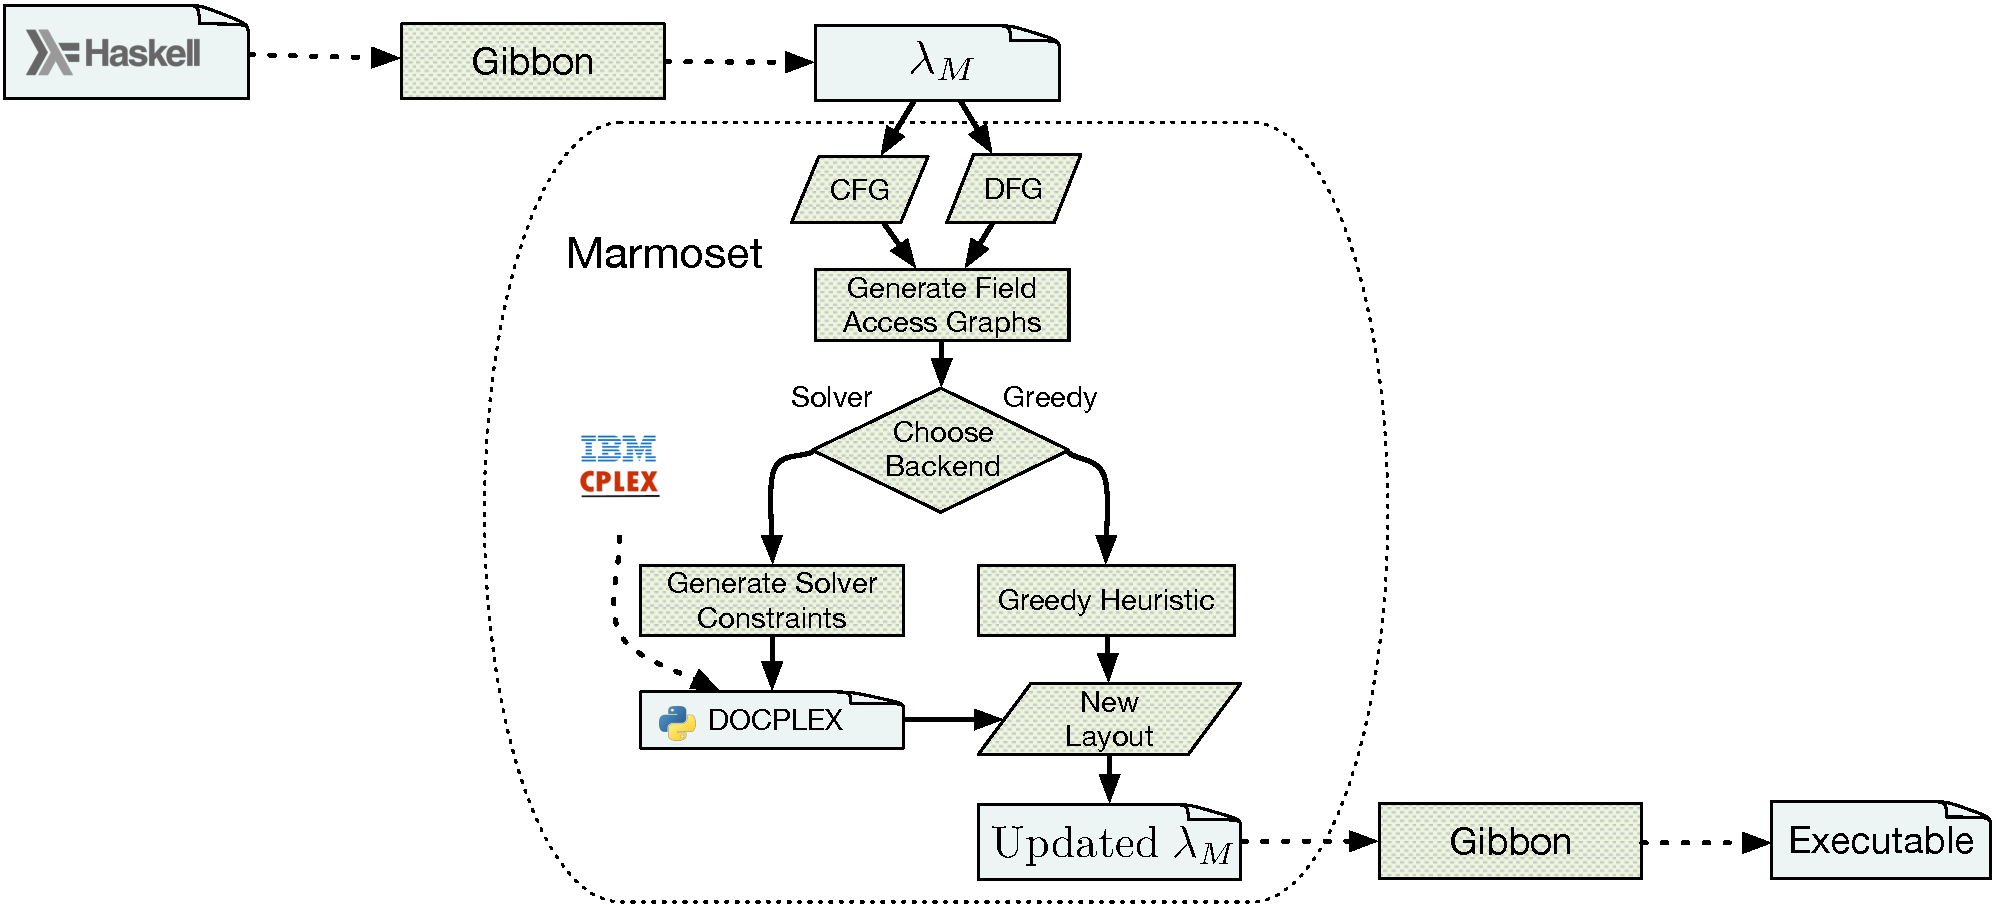
\includegraphics[scale=0.4]{figures/OverallPipeline2}
	\caption{The overall pipeline of \system.}
	\label{figure:overall-pipeline}
\end{figure}
%
The Gibbon front-end uses standard whole-program compilation and monomorphization techniques~\cite{urweb-icfp}
to lower input programs into a first-order, monomorphic IR (\systemlang{}).
%
Gibbon performs location inference on this IR to convert it into a LoCal program,
which has regions and locations, essentially, buffers and pointer arithmetic.
%
Then a big middle section of the compiler is a series of LoCal $\rightarrow$ LoCal compiler passes that
perform various transformations.
%
Finally, it generates C code.
%\csk{perhaps this paragraph is unnecessary, but we don't say much about gibbon anywhere else.}
Our extension operates towards the front-end of the compiler, on \systemlang{}.
%
We closely follow the design described in Section~\ref{sec:design} to construct the
control-flow graph and field-access graph, and use the standard Haskell graph library\footnote{https://hackage.haskell.org/package/containers} in our implementation.

To solve the constraints, we use IBM's DOCPLEX (Decision Optimization CPLEX),
because its API allows high level modelling such as logical expressions like implications, negations, logical AND etc. with relatively low overhead. 
%
%% via its Python bindings
Unfortunately, there isn't a readily available Haskell library that can interface with DOCPLEX.
%
Thus, we use it via its library bindings available for Python.
%
Specifically, we generate a Python program that feeds the constraints to DOCPLEX and
outputs an optimum field ordering to the standard output,
which \system{} reads and parses, and then reorders the fields accordingly.
%
% The field ordering is output as a list of tuples, \il{[(Int, Int)]},
% where the first component is the original field index and the second component
% is that field's new index.

%% %
%% In the remainder of this section we outline 

% \mv{Do you need an implementation section, or can you just explain the implementation in the design section?}

% %% \subsection{Using an ILP solver to solve the generated constraints}
% \subsection{Solving Cost Model Constraints}
% \label{design:ilp}

% %% \vs{ILP solver.}

% We construct the field access graph and ILP (integer linear program) as detailed in Section~\ref{sec:design}. The abstract cost model works with four costs, subject to the constraints in Equation~\ref{eq:costs}. Because every term of the objective function (Equation~\ref{eq:objective}) is a multiple of one of these costs, the only thing that matters is the relative values of the costs, not their absolute value. Hence, we use a ratio of 1:2:3:4 for $C_\mathit{succ}$, $C_\mathit{after}$, $C_\mathit{pred}$ and $C_\mathit{before}$, respectively in case of a data flow edge. In case of a control flow edge, it depends on the attribute of the fields but the costs are integral multiples of each other. 

% \new{After constructing the ILP,
% we use a commercially available ILP solver, CPLEX~\cite{cplex},
% to obtain a minimum-cost ordering.}
% %% generated the constraints using the access graph $G$, we can directly generate code for these constraints targeted for a commercially available ILP solver.
% %
% The logical constraints described in section~\ref{design:genconstraints} cannot directly be given as an input to CPLEX.
% %% in a trivial ILP solver.
% %% However, we there are various known techniques to linearize these logical expressions to work with 
% %% %% work for a vanilla ILP solver.
% %% We show the linearized versions of these constraints in the appendix of our extended paper. 
% %
% To solve these constraints, we use IBM's DOCPLEX (Decision Optimization CPLEX),
% because its API allows high level modelling such as logical expressions like implications, negations, logical AND etc. with relatively low overhead. 
% %
% %% via its Python bindings
% Unfortunately, there isn't a readily available Haskell library that can interface with DOCPLEX.
% %
% Thus, we use it via its library bindings available for Python.
% %
% Specifically, we generate a Python program that feeds the constraints to DOCPLEX and
% outputs an optimum field ordering to the standard output,
% which \system{} reads and parses, and then reorders the fields accordingly.
% %
% The field ordering is output as a list of tuples, \il{[(Int, Int)]},
% where the first component is the original field index and the second component
% is that field's new index.

%% we use a staging compiler that uses the \textit{language-python} library in haskell to automatically generate python code for IBM's DO (decision optimization) CPLEX~\cite{cplex} library. 
%% %
%% We specifically use DOCPLEX since its object oriented API allows high level modelling (such as logical expressions like implications, negations, logical AND etc.) with relatively low overhead. 
%% %
%% The DOCPLEX solver gives us a mapping from the old fields of the data constructor to the new index positions in the data constructor that locally optimize the performance of traversal $\FD$. We use this index map to re-order the fields in the data constructor and repair the code which we talk about next.   

% \subsection{Reordering Fields of a Datatype}
% \label{design:shufflefields}

% Once we obtain an optimum field ordering for a specific data constructor globally, we update that data constructor to have this new field order.
% %
% %% The ILP solver returns the new field ordering for the data constructor and function pair we are trying to locally optimize the program for. We use this field order to change the instantiated order of fields of the corresponding data constructor ($\sDC$) of value type $T$.
% Consequently, we need to repair the complete program to adhere to the updated data constructor.

%% A
%% % \textit{L1}
%% compiler pass, operating on the \systemlang{} IR, uses the optimal field ordering to permute the fields of the data constructor $d$ and modifies its type $T'$. We then recursively traverse each function and permute the case bindings and all expressions where the data constructor $\sDC$ is being written to so that the program type checks. Doing so ensures that we generate correct code. Performing this transformation
%% % at the \textit{L1} level
%% early in the compiler
%% is beneficial since downstream compiler passes like \textit{inferLocations}
%%   (which does the major work of converting to location calculus)
%% are able to implement the serialized data operations just as if the
%% programmer had writen the desired the data layout in the original source code of their program.
%% %% correctly reason about the region and location calculus as if the programmer instantiated the correct layout at the top level.
%% % \mv{This sentence is likely to not be understood by a reader unfamiliar with LoCal.}

% % \subsection{Using annotation pragmas to allow the user to specify various constraints over the fields of a data constructor.}
% \subsection{Annotation Pragmas for Optional, Manual Ordering Constraints}
% \label{sec:annotation-pragmas}
% %% \vs{Annotation pramas to give the user control to define the layout of fields + different kinds of constraints and how contraints are generated for the them.}
% %


% % -- User requsets the compiler optimize the Cons constructor
% % -- based on the access patters of fields in traversal foo.
% % {-# ANN foo Cons #-}

% \begin{figure}% [H]
% 	\begin{lstlisting}[]
       
%                 -- User defines some absolute constraints as assignments of field indices.
% 		{-# ANN Cons (foo, (0 ~> 3, 1 ~> 2)) #-}    
		
% 		-- User defines some relative (``after'') constraints.
% 		{-# ANN Cons (foo, (4 :> 5, 3 :> 2)) #-}
		
% 		data List = Nil | Cons F0 F1 F2 F3 F4 F5 List

% 		foo :: List -> List 
% 		foo lst = case lst of 
% 		                Cons f1 f2 f3 f4 f5 f6 rst -> ...

% 	\end{lstlisting}
% 	\caption{User annotations in \system to define constraints over fields of a data constructor. The annotations are defined as ANN annotations for a specific function and data constructor that function uses. }
% 	\label{fig:userAnnotations}
% \end{figure}

% Optional, manual control over data layout has uses beyond second guessing the automatic optimizer.
% %% Allowing users to specify constraints over the layout of fields in a data constructor is a useful capability. This allows the user to match the layout of the data constructor to certain specifications they may have.
% %
% For instance, the user may wish to store the data in a certain format on disk or provide information for ordering that may affect performance downstream for reasons the user has information about. In addition, the user may want to read existing data in a certain format residing on disk. We allow the user to specify the layout of fields in \system through annotations (pragmas). Currently, our compiler allows these specifications to be defined for a specific function and data constructor[s].
% %% However, we plan to extent our model to specify these constraints for multiple functions and even globally across functions.
% %
% We allow the user to specify two kinds of constraints over the fields of a data constructor. These are shown in figure~\ref{fig:userAnnotations}. 

% \begin{itemize}
% \item \textbf{Absolute Constraints:} These constraints allow the user to specify an exact position for a field in a data constructor. The \textit{ANN} annotation names a specific data constructor, a function name, and a list of field (indices) as well as their assigned positions.
% % $Cons (foo, (0 \sim~> 3))$ says to   
% %%   contains the data constructor to be optimized and the tuple contains the function name followed by the ordering specified in the inner tuple. The ordering in the nested (inner) tuple uses a special infix operator ``$\sim>$'' to determine the new index position for the field in the index on the left hand side of the infix operator.
%   Hence $0 \sim> 3$ in the ANN annotation assigns the field at position $0$ to position $3$ in the data constructor. This is parsed by the compiler and added as metadata in the function body
%   % of the function the ordering is defined for.
%  The constraint solver honors these constraints, while freely moving around the other fields.
% For example, $0 \sim> 3$ will generate the following constraints in the constraint solver :  ${F0}_{index} = 3$

% \item \textbf{Relative Constraints:} These constraints allow the user to specify the relative ordering of fields in a data constructor. Currently we support ``Immediately After'' constraints but these can be extended to other types of relative constraints in the future. Immediately After constraints allow the user to place one field right after another one. For instance, ``$4 :> 5$'' can be interpreted as placing field at index position $4$ right after the field at index position $5$. Such a specification by the user will generate the following constraint in the constraint solver : ${F4}_{index} = {F5}_{index} + 1$ for the example shown in figure~\ref{fig:userAnnotations}.

% % \item \textbf{Activating optimization:}
% % \item \textbf{Optimization Hints:}
% %   \new{The user can specifically invoke \system on a particular combination of function and data constructor(s).
% % %
% %     This is a hint from \system to process the function, and may be subsumed by future strategies that automatically apply (and cache solver results for) the optimization.
% % %
% %  In any case, the performance optimization search previously described
% %  will always respect any other hard constraints that have been
% %  annotated.}
  
% % \item \textbf{Soft Constraints (automatic performance optimization):}
% % 
% %% The user can specify the automatic layout optimization for performance using yet another ANN annotation pragma shown in figure~\ref{fig:userAnnotations}. This instructs \system to perform the automatic optimization for a specific function and data constructor that we have already discussed. We call these generated constraints defined in section~\ref{design:genconstraints} as ``soft constraints''. They are called soft since they do not impose a strict ordering as would be by the absolute and relative constraints but is rather driven by the costs induced by the access patterns of the traversal. These constraints would essentially take a back seat if the user has defined a stricter constraint for a field used in the function body. However, these can work in tandem with the strict orderings(if provided) to better optimize the layout for the traversal. In the absence of user specified relative and absolute orderings, \system will optimize the layout for performance as discussed before.

% \end{itemize}


